\documentclass[11pt,a4paper]{article}
\usepackage[margin=2.5cm]{geometry}
\usepackage{graphicx}
\title{Labwork 8: Scatter}
\author{Duong Tan Binh \\ Student ID: 2540007}
\date{}
\begin{document}
\maketitle
\section{RGB to HSV}
I use the RGB image from Lab 3. Each 2D thread divides its three channels
by 255 and applies the formulas in the slide. Hue is in degrees;
saturation and value are between 0 and 1.
I store H, S and V in three separate arrays instead of keeping three
channels together for each pixel. For gray pixels I set hue to 0;
for black pixels I also set saturation to 0.

\section{HSV to RGB}
I follow the slide: \texttt{d = H / 60}, \texttt{hi = int(d) mod 6},
then \texttt{l}, \texttt{m} and \texttt{n}. The value of \texttt{hi}
tells which of the six cases is used for R, G and B.
I multiply by 255, round to the nearest integer and keep values in 0 to 255.
Both kernels use 16 by 16 blocks and check image boundaries.

\section{Comparison}
\begin{verbatim}
Maximum channel difference: 0
Different pixels: 0
\end{verbatim}
The restored image matches the input exactly in this test.
I compare decoded pixels and save the output as PNG to avoid JPEG changes.


\begin{center}
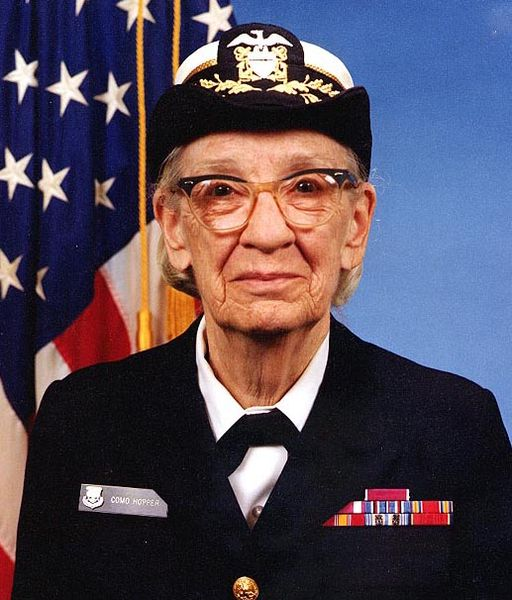
\includegraphics[width=0.40\textwidth]{input.jpg}
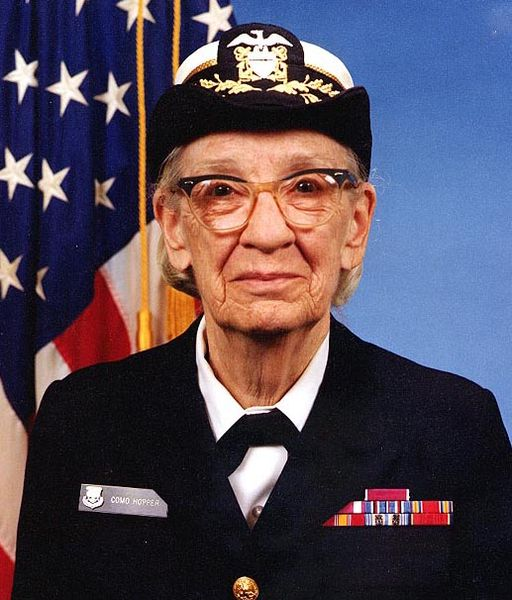
\includegraphics[width=0.40\textwidth]{restored.png}
\end{center}
Input RGB image and RGB image restored from HSV.

\end{document}
